\subsection{Assigned Race List}
\subsubsection{Class Diagram}
 
\begin{figure}[H]
    \centering
    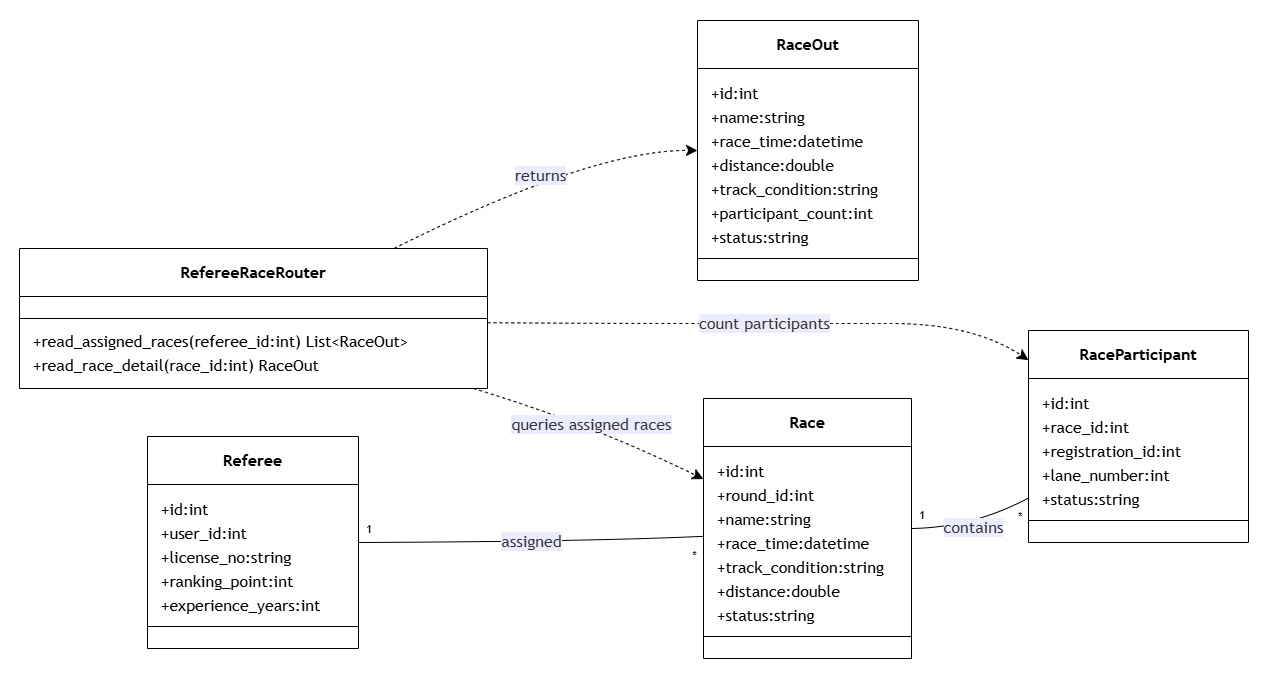
\includegraphics[width=\textwidth,height=0.78\textheight,keepaspectratio]{figures/design/referee/Assigned_Race_List_class.png}
    \caption{Assigned Race List Class Diagram}
    \label{fig:assigned_race_list_class_diagram}
\end{figure}
 
\subsubsection{Sequence Diagram}
 
\begin{figure}[H]
    \centering
    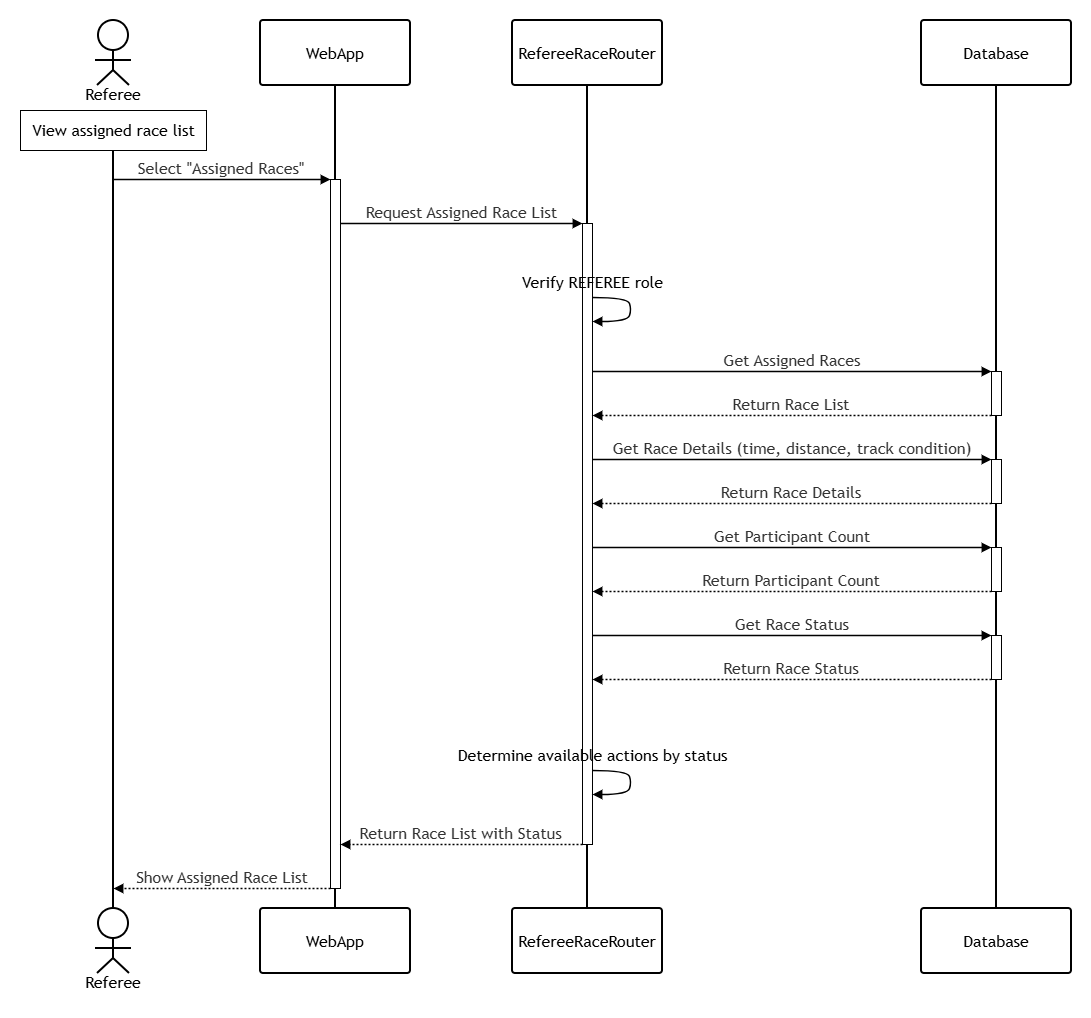
\includegraphics[width=\textwidth,height=0.78\textheight,keepaspectratio]{figures/design/referee/Assigned_race_list_seq.png}
    \caption{Assigned Race List Sequence Diagram}
    \label{fig:assigned_race_list_sequence_diagram}
\end{figure}
 
\subsubsection{Class Specification}
 
\begingroup
\small
\setlength{\tabcolsep}{3pt}
\TableStart{|>{\raggedright\arraybackslash}p{0.25\textwidth}|>{\raggedright\arraybackslash}p{0.31\textwidth}|>{\raggedright\arraybackslash}p{0.14\textwidth}|>{\raggedright\arraybackslash}p{0.25\textwidth}|}
\textbf{Class} & \textbf{Attributes / Methods} & \textbf{Type} & \textbf{Description} \\
\hline
Referee\allowbreak{}Race\allowbreak{}Router & read\_assigned\_races(), read\_race\_detail() & controller / route & Handles HTTP requests to retrieve the list of races assigned to the authenticated referee and their details. \\
\hline
RaceOut & id, name, race\_time, distance, track\_condition, participant\_count, status & DTO & Output data transfer object returning summarized race information for the referee's assigned race list. \\
\hline
Race & id, round\_id, name, race\_time, track\_condition, distance, status & entity & Database entity storing core information of a horse racing event. \\
\hline
Race\allowbreak{}Participant & id, race\_id, registration\_id, lane\_number, status & entity & Database entity representing a registered horse and jockey combination participating in a race, used to compute participant count. \\
\hline
Referee & id, user\_id, license\_no, ranking\_point, experience\_years & entity & Database entity storing role-specific information of the race referee, including licensing and assignment eligibility. \\
\TableFinish{Assigned Race List class specification}{tab:assigned_race_list_class_spec}
\endgroup
 
\subsection{Race Inspection}
\subsubsection{Class Diagram}
 
\begin{figure}[H]
    \centering
    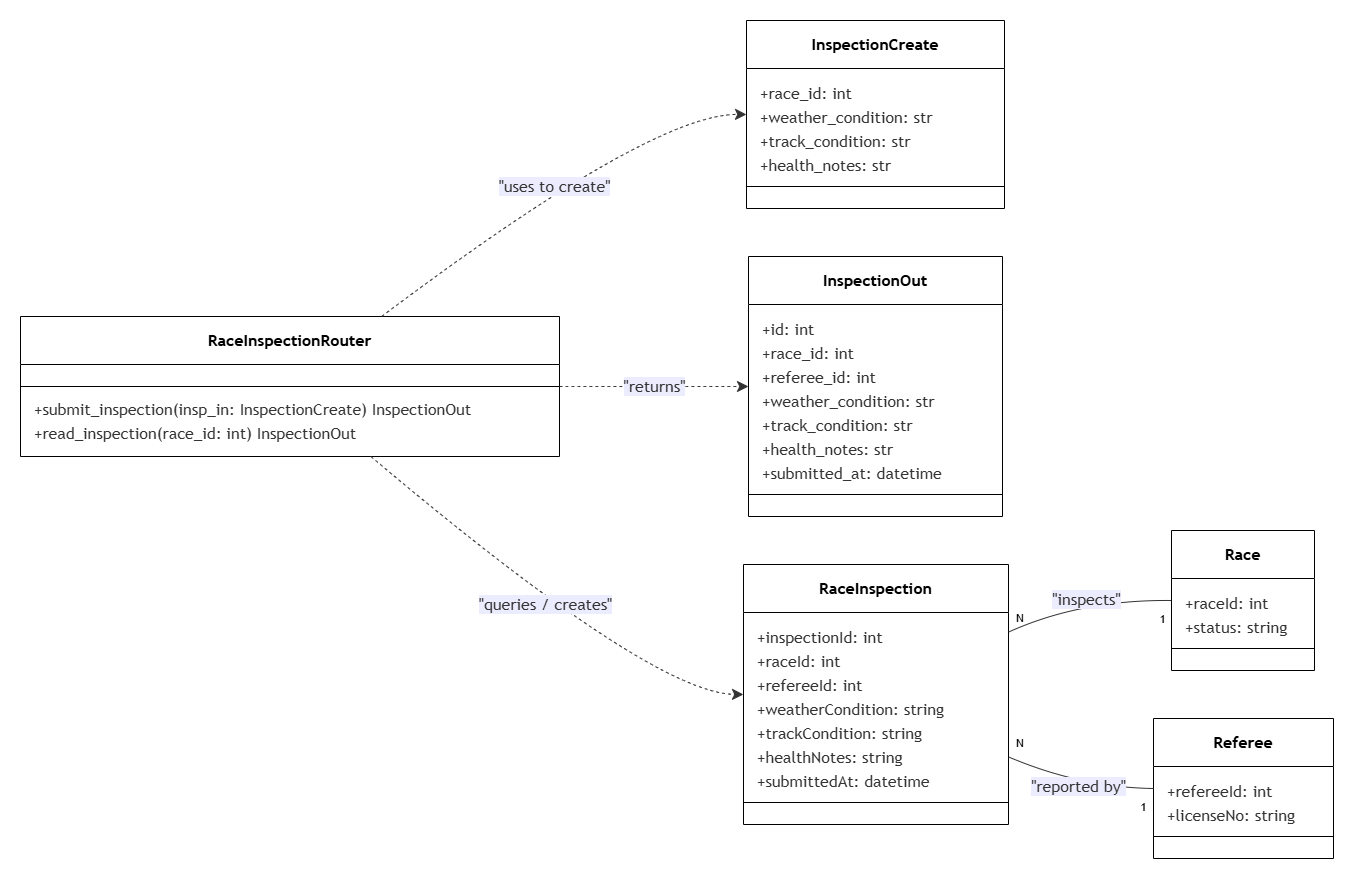
\includegraphics[width=\textwidth,height=0.78\textheight,keepaspectratio]{figures/design/referee/Race_Inspection_class.png}
    \caption{Race Inspection Class Diagram}
    \label{fig:race_inspection_class_diagram}
\end{figure}
 
\subsubsection{Sequence Diagram}
 
\begin{figure}[H]
    \centering
    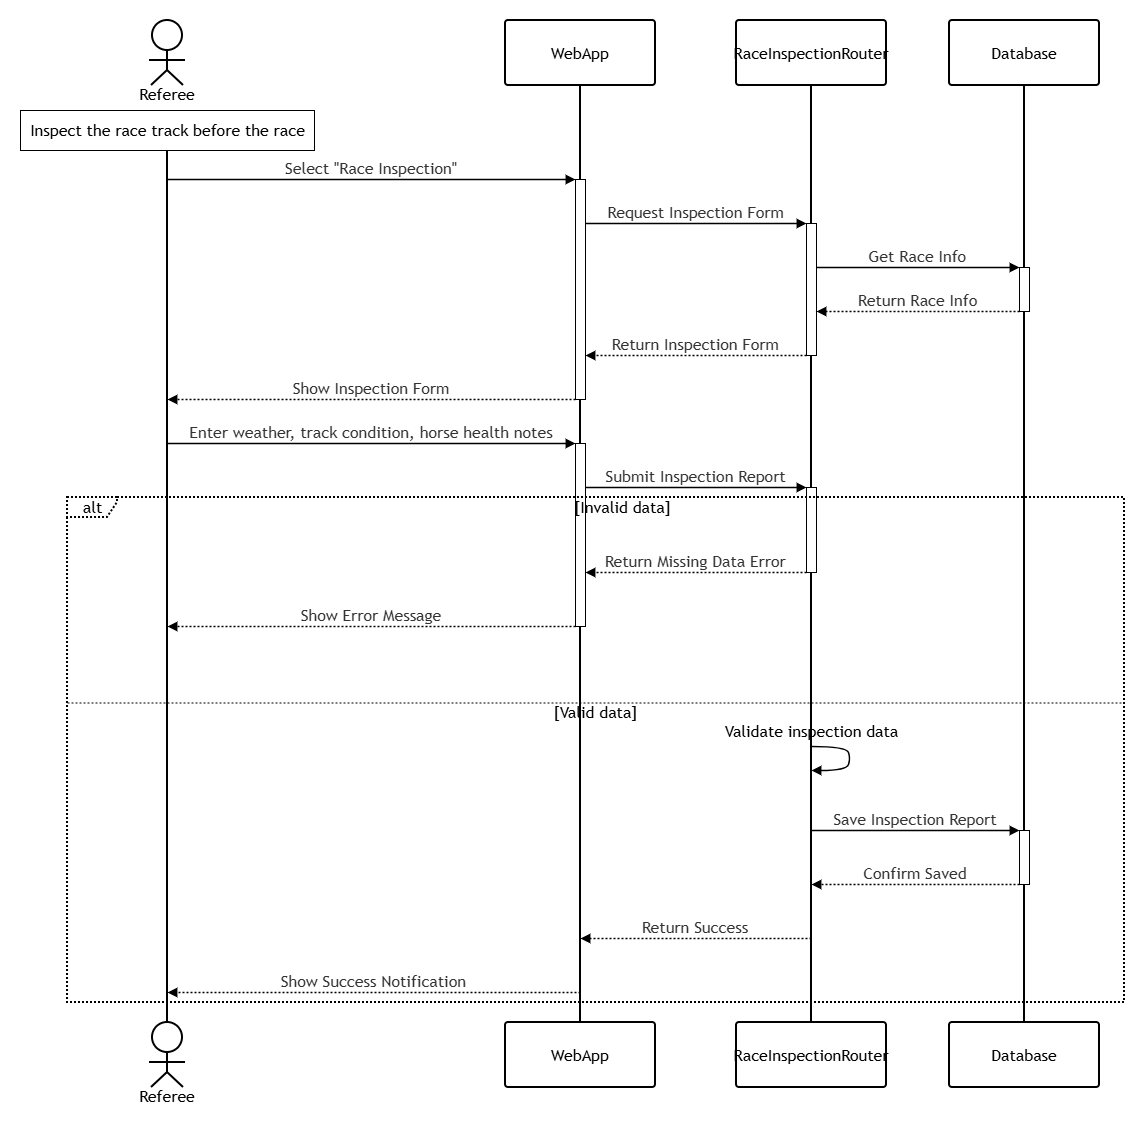
\includegraphics[width=\textwidth,height=0.78\textheight,keepaspectratio]{figures/design/referee/Race_inspection_seq.png}
    \caption{Race Inspection Sequence Diagram}
    \label{fig:race_inspection_sequence_diagram}
\end{figure}
 
\subsubsection{Class Specification}
 
\begingroup
\small
\setlength{\tabcolsep}{3pt}
\TableStart{|>{\raggedright\arraybackslash}p{0.25\textwidth}|>{\raggedright\arraybackslash}p{0.31\textwidth}|>{\raggedright\arraybackslash}p{0.14\textwidth}|>{\raggedright\arraybackslash}p{0.25\textwidth}|}
\textbf{Class} & \textbf{Attributes / Methods} & \textbf{Type} & \textbf{Description} \\
\hline
Race\allowbreak{}Inspection\allowbreak{}Router & submit\_inspection(), read\_inspection() & controller / route & Handles HTTP requests related to submitting and retrieving pre-race inspection reports. \\
\hline
Inspection\allowbreak{}Create & race\_id, weather\_condition, track\_condition, health\_notes & DTO & Input data transfer object used to submit a new race inspection report. \\
\hline
Inspection\allowbreak{}Out & id, race\_id, referee\_id, weather\_condition, track\_condition, health\_notes, submitted\_at & DTO & Output data transfer object returning the submitted inspection report details. \\
\hline
Race\allowbreak{}Inspection & id, race\_id, referee\_id, weather\_condition, track\_condition, health\_notes, submitted\_at & entity & Database entity storing the referee's pre-race inspection findings for a given race. \\
\hline
Race & id, round\_id, name, race\_time, track\_condition, distance, status & entity & Database entity storing core information of the race being inspected. \\
\hline
Referee & id, user\_id, license\_no & entity & Database entity identifying the referee who submitted the inspection report. \\
\TableFinish{Race Inspection class specification}{tab:race_inspection_class_spec}
\endgroup